\documentclass{paper}
\usepackage[margin=0.5in]{geometry}
\usepackage{graphicx}
\usepackage{listings}

% \includegraphics[scale=1]{img.png}
% \begin{lstlisting} 
\title{8. Linux Input Drivers}
\begin{document}
\maketitle
\line(1,0){510}
\begin{itemize}
\item \textit{Hvad d\ae kker begreberne Input Device Driver og Input Event Driver over?}
\item \textit{Hvad er evdev?}
\item \textit{Eksempler p\aa\ input event driver typer?}
\item \textit{Eksempel p\aa\ hvilke elementer som en virkelig(f.eks. touch screen) driver indeholder og hvordan de h\ae nger sammen. Interrupt, spi etc\\}
\end{itemize}

\begin{large}\textbf{Hvad d\ae kker begreberne \textit{Input Device Driver} og \textit{Input Event Driver} over?}\end{large}\\
\line(1,0){510}
\begin{itemize}
\item \textbf{Input Device Driver:}
	\begin{itemize}
	\item S\o rger for interaktion mellem enheden og kernen
	\end{itemize}
\item \textbf{Input Event Driver:}
	\begin{itemize}
	\item S\o rger for interaktion mellem userspace applikationer og kernen\\
	\end{itemize}
\end{itemize}

\begin{large}\textbf{Hvad er evdev?}\end{large}\\
\line(1,0){510}
\begin{itemize}
\item Et kernel under-system der s\o rger for ensartet kommunikation mellem input devices og userspace(X-server, gpm)
\item Laver et ensartet interface til alle input devices
\item Keyboards, joysticks, touchscreens, mus osv.\\
\end{itemize}

\begin{large}\textbf{Eksempler p\aa\ input event driver typer?}\end{large}\\
\line(1,0){510}
\begin{itemize}
\item Keyboards, joysticks, touchscreens, mus osv.\\
\end{itemize}
\begin{large}\textbf{Eksempel p\aa\ hvilke elementer som en virkelig(f.eks. touch screen) driver indeholder og hvordan de h\ae nger sammen. Interrupt, spi etc}\end{large}\\
\line(1,0){510}
\begin{itemize}
\item Touch screen output er tilkoblet SPI
\item Der interruptes
\item SPI overf\o rer information om coordinater
\item evdev informeres om disse:
\begin{lstlisting}
input_report_rel(input_dev, REAL_X, x);

input_sync(input_dev);
\end{lstlisting}
\item Gentag
\end{itemize}

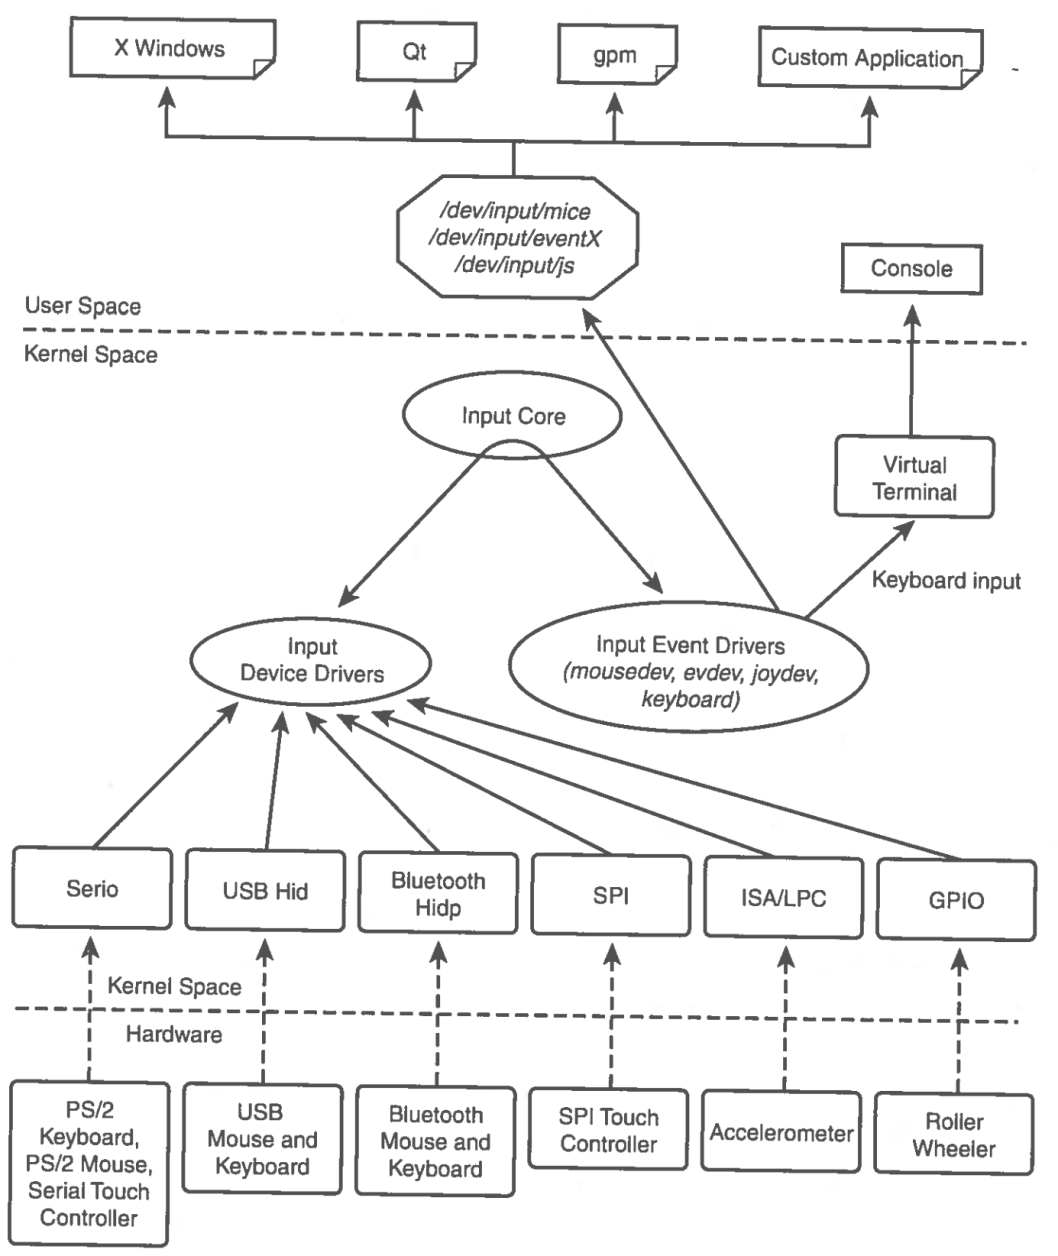
\includegraphics[scale=1,angle=0.72]{inputsys.png}
\end{document}
